\section{Abstract Translation Algorithm}
\label{sec:AbstractTranslation}

Our approach for abstract traslation borrows the idea of reusing the control structures used in 
classical parsing from~\cite{AbstrParsing}. Control tables of LALR analyzer may be generated by
some conventional tool (e.g. yacc\footnote{http://dinosaur.compilertools.net}). The interpreting 
automaton, however, has then to be modified to be able to compute all possible parser states 
for each vertex of the input graph. 

%So, the basic idea of the abstract parsing is a graph processing with fix-point calculation~\cite{ALVOR2}.

For example, let we have the following grammar:

\begin{verbatim}
   s -> Ae
   e -> BD
   e -> CD
\end{verbatim}

An input graph is shown on the Fig.~\ref{pic2}. The set of parser states for each vertex of 
the graph can be calculated during syntax analysis. The result of state calculation is shown on 
the Fig.~\ref{pic3}.

\begin{figure}
    \begin{center}
        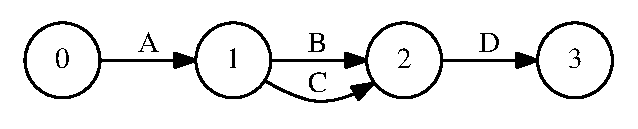
\includegraphics[width=7cm,height=1.5cm]{graphs/simple_grammar_inpt.eps}
        \caption{Input graph for abstract parsing}
        \label{pic2}
    \end{center}
\end{figure}

\begin{figure}
    \begin{center}
        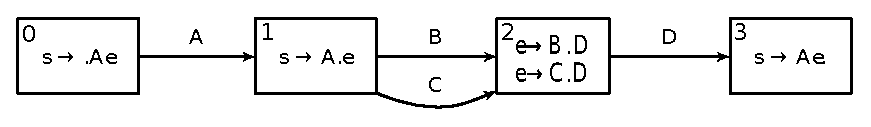
\includegraphics[width=11cm,height=1.5cm]{graphs/simple_grammar_items.eps}
        \caption{Parser states}
        \label{pic3}
    \end{center}
\end{figure}

%So, there is an algorithm for syntax analysis of string-embedded languages. Note, that the problem of static 
%analysis if dynamically generated strings could not be solved in the common case~\cite{ALVOR2}. Also there are 
%possible two implementation of abstract parsing algorithm except our one. Note that these tools do not solve 
%the problem of string-embedded statements translation.

In the case of translation (not parsing) the parsing state consists of state of the automaton and some
\emph{semantic} value which represents the result of translation built so far. In particular,
the translation algorithm works not only with token types, but also tolen values. 

%
%It is possible to merge states like in GLR-algorithm\cite{Grune}. This way we can avoid problems with size of states set and parsing result.
%If we want to translate input expression to another language then we should keep all information 
%about tokens values. 

%We propose to modify basic LALR-based algorithm of abstract parsing to solve the problem of abstract 
%translation. The original parsing algorithm targeted to recognition, not translation, and it does not 
%support semantics calculation. This fact allows to operate only with tokens type, not tokens values. 

One of the possible solution of translation is abstract parsing algorithm with mechanism of stack 
splitting for semantic calculation support. It disallows to merge states and creates a new 
copy of the whole stack for the each branch of the input graph.

However, this approach faces the exponential memory usage problem. 
% Note that there is a big number of dynamic expressions which require exponential resources to 
%analyze in the real world information systems. 
For example parser states for vertex $V_3$ on the Fig.~\ref{pic4} should be equal for two input edges
but if we want to calculate semantics, then we get two different states because identifiers has 
different values.

\begin{figure}
    \begin{center}
        \includegraphics[width=9cm,height=1.1cm]{graphs/states_example.eps}
        \caption{Graph with states possible to merge}
        \label{pic4}
    \end{center}
\end{figure}

Queries which contain a huge number of branches is a big problem. The number of states is an 
exponential function of the number of branches because for each branch we should produce $n*k$ 
states where $n$ is a number of states in the root of the fork vertex and $k$ is the number 
of branches. One of the most frequent example of queries with big number of branches 
is \verb|select| query. Each of fields to select can be calculated with if-statement 
or case-statement. Example of such graph is presented on the Fig.~\ref{pic5}.

\begin{figure}
    \begin{center}
        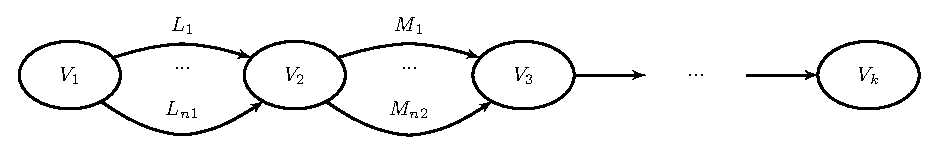
\includegraphics[width=7.7cm,height=1.5cm]{graphs/big_res.eps}
        \caption{Graph which requires an exponential resources for translation}
        \label{pic5}
    \end{center}
\end{figure}

If we use only sequentially concatenated if-statements then the number of parsing trees is $2^n$ 
where $n$ is a number of if-statements (or number of branches). In some real-world systems we 
have faced the queries which contains more than 100 branches. The full forest calculation by naive 
adaptation of abstract parsing is impossible for such queries. 

%The set of states to be processed
%minimization is an actual problem for real-world systems.

%\subsection{Optimization of the abstract translation algorithm}
%\label{sec:Optimizations}

We propose the following solution for the forest size minimization problem. We have previously mentioned 
that the result of translation is a new values for all variables which were used for queries construction. 
It is sufficient to construct not the full forest but only the minimal set of trees such that after 
translation every variable gets new value.This way, we can process not all paths in the input graph 
but only minimal set which contains all edges. Note that we cannot calculate this set prior to the parsing 
because we cannot be sure that every path produces syntactically correct value. If some path contains 
error than the tree for that path is not constructed and we may lose information about variables. 
For example consider the graph presented on the Fig.~\ref{pic6}.

\begin{figure}
    \begin{center}
        \includegraphics[width=4.8cm,height=1.2cm]{graphs/paths.eps}
        \caption{Graph for minimal paths set selection.}
        \label{pic6}
    \end{center}
\end{figure}

The one possible set of paths which we can calculate before syntax analysis is $\{(L_1; M_1); (L_2; M_2)\}$. 
But every path here contains syntax errors and the result forest would be empty instead of containing 
two trees. We should choose another set (for example $\{(L_1; M_2); (L_2; M_1)\}$) to get the correct result. 

So, path calculation is an iterative process. We perform state filtering during syntax analysis for each vertex 
with multiple input edges. Let describe the steps of the process:

\begin{itemize}
    \item \textbf{Initial state.} Set of states for the vertex is empty. 
    \item \textbf{Step.} For each step if the current vertex has multiple input edges then we should add new 
                 state to a state set for the current vertex if one of the following conditions is true:
    \begin{itemize}
        \item new state corresponds to a path, which contains some edges which are not contained in any of the paths, which correspond to any state of the currently processing set;
        \item new state corresponds to a parser state which is not yet presented in the currently processing set.
    \end{itemize}

\end{itemize}

\begin{comment}
Described algorithm pseudo code is presented below.
\begin{verbatim}
/*
V – list of input graph vertices in the topological order.
v_s – start vertex of input graph.
*/

let filterStates v =
    let groupedByParserState =
        v.States.GroupBy (fun state -> state.Item)

    v.States = Set.empty

    for group in groupedByParserState do
        /* Each state corresponds with path from v_s to v.
         Set of paths specify set of edges of graph E_s.
         We should construct minimal set of paths which
         contains all edges of E_s. The next greedy algorithm
         can be applied to solve this problem.
         1) Order paths by length ascent.
         2) While current path contains edges not in
         the result set add this path in the result set.*/
        let ordered = 
            group.OrderBy (fun s -> -1 * s.Path.Lenght)
        for s in ordered do
            if (s.Path contains edges which 
                not in any path from result set) 
            then v.States.Add s

for v in V do
    v.States <- … /*step of syntax analysis*/
    /*If input degree of the vertex v more 
      then 1 then try to filter states.*/
    if v.InEdges.Count > 1 then filterStates v

\end{verbatim}
\end{comment}

This way we can get state set which contains all parser states from input set but is not greater 
than it. Corresponding paths contain all possible edges in processed subgraph. Described algorithm
of filtration allows to increase the performance of parsing by decreasing the number of parsing trees.
